\documentclass[conference]{IEEEtran}
\IEEEoverridecommandlockouts%

\usepackage[utf8]{inputenc}
\usepackage[T1]{fontenc}
\usepackage[english,brazilian]{babel}
\usepackage{amsmath}
\usepackage{array}
\usepackage{booktabs}
\usepackage{graphicx}
\usepackage{bookmark}
\usepackage{eso-pic}
\usepackage[section]{placeins}
\usepackage{tikz}
\usepackage{hyperref}
\usepackage{url}

\hypersetup{colorlinks=true,linkcolor=blue,urlcolor=blue,citecolor=blue}

\AddToShipoutPictureBG{%
\begin{tikzpicture}[remember picture,overlay]
\node[opacity=0.06,inner sep=0pt] at (current page.center) {
\includegraphics[width=0.48\paperwidth]{figures/unb-logo-square.png}};
\end{tikzpicture}%
}

\title{%

\includegraphics[width=0.95\textwidth]{figures/unb-logo-wide.jpg}\\[-0.8ex]
\vspace{0.4ex}
Plataforma Web em Tempo Real para Monitoramento, Telemetria e Comparação de TCP e UDP}

\author{%
\IEEEauthorblockN{Navinchandry Bittencourt Ruas}
\IEEEauthorblockA{Departamento de Ciência da Computação\\
Universidade de Brasília\\
Matrícula: 241034353\\
241034353@aluno.unb.br}
}

\begin{document}
\maketitle

\begin{abstract}
Este relatório apresenta o NetPulse, uma aplicação web simples desenvolvida para demonstrar conceitos de redes de computadores por meio de comunicação HTTP, WebSocket, TCP e UDP.\@ A solução implementa autenticação de usuários, envio e persistência de telemetria, alertas automáticos, atualização em tempo real e um módulo de benchmark para medir RTT e throughput. Também são descritos o protocolo de aplicação, o ambiente experimental e a estratégia de análise com Wireshark. A proposta prioriza reprodutibilidade em laboratório e execução local estável.
\end{abstract}

\noindent Palavras-chave: redes de computadores, HTTP, WebSocket, TCP, UDP, monitoramento em tempo real

\vspace{1\baselineskip}

\begin{otherlanguage}{english}
\begin{abstract}
This report presents NetPulse, a simple web application designed to demonstrate computer networking concepts through HTTP, WebSocket, TCP, and UDP communication. The solution includes user authentication, telemetry submission and persistence, automatic alerts, real-time updates, and a benchmark module for measuring RTT and throughput. It also describes the application protocol, the experimental environment, and the Wireshark-based analysis strategy. The proposal prioritizes laboratory reproducibility and stable local execution.
\end{abstract}
\noindent Keywords: computer networks, HTTP, WebSocket, TCP, UDP, real-time monitoring
\end{otherlanguage}

\section{Introdução}
O projeto NetPulse foi desenvolvido no contexto da disciplina de Redes de Computadores com o objetivo de materializar, em uma aplicação funcional, os conceitos de comunicação fim a fim, encapsulamento, multiplexação e análise de protocolos~\cite{tanenbaum,kurose}. A proposta atende aos requisitos do roteiro ao combinar interface web, servidor de aplicação, persistência local, comunicação em tempo real e comparação entre TCP e UDP.\@

\section{Fundamentação Teórica}
Aplicações em rede normalmente combinam diferentes protocolos de transporte e aplicação para equilibrar confiabilidade, latência e complexidade. Em NetPulse, o HTTP é usado como protocolo principal de interação entre navegador e servidor, pois simplifica autenticação, cadastro e envio de telemetria~\cite{rfc9110}. O WebSocket complementa essa camada ao manter uma conexão persistente para atualizações em tempo real~\cite{rfc6455}.

TCP e UDP foram adotados para ilustrar comportamentos distintos na camada de transporte. O TCP fornece entrega confiável, controle de fluxo e estabelecimento de conexão por meio do handshake de três vias, enquanto o UDP prioriza simplicidade e baixa sobrecarga, não garantindo entrega nem ordenação~\cite{rfc793,rfc768}. Em Wireshark, essa diferença aparece no formato dos pacotes, na sequência observada e na presença ou ausência de retransmissões~\cite{wireshark}.

\section{Ambiente Experimental e Análise de Resultados}
\subsection{Descrição do Cenário}
O experimento foi concebido para execução local em ambiente de laboratório, usando um cliente web acessado no navegador e um servidor Node.js que expõe HTTP, WebSocket, TCP e UDP.\@ A topologia é de loopback, o que reduz ruído externo e facilita a inspeção dos pacotes capturados em interfaces locais. Essa decisão também permite reproduzir o experimento em máquinas diferentes sem dependência de infraestrutura adicional.

\begin{itemize}
\item \textbf{HTTP}: autenticação, cadastro, envio de telemetria e requisição dos benchmarks.
\item \textbf{WebSocket}: atualização assíncrona do painel com alertas, telemetria e logs.
\item \textbf{TCP/UDP}: relays de transporte usados para gerar tráfego analisável no Wireshark e comparar RTT e throughput.
\end{itemize}

\begin{figure}[!htbp]
\centering
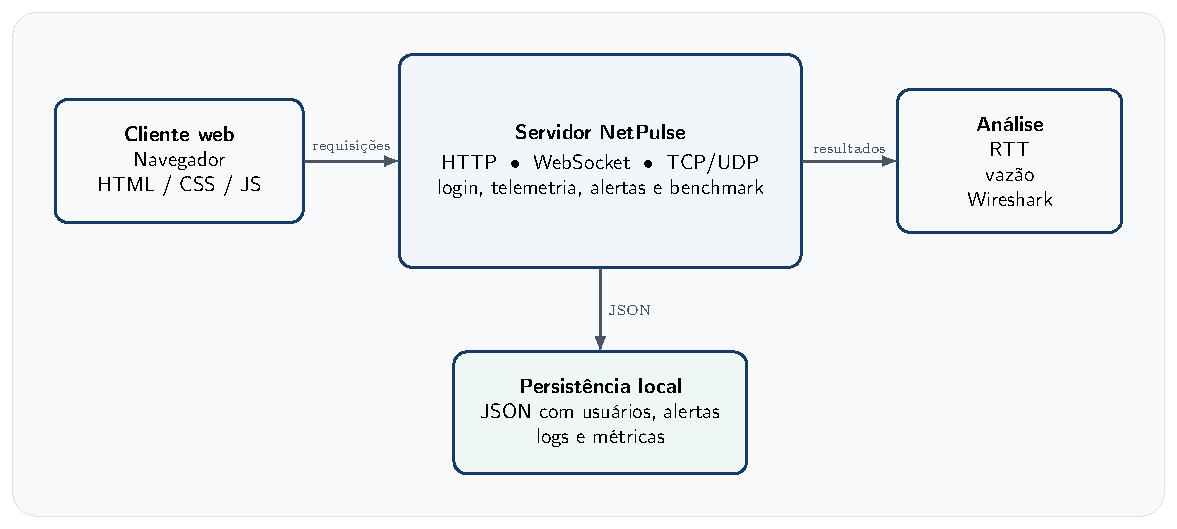
\includegraphics[width=0.98\linewidth]{figures/fig1-architecture.pdf}
\caption{Arquitetura geral do NetPulse e seus canais de comunicação.}\label{fig:architecture}
\end{figure}

O protocolo de aplicação do NetPulse utiliza JSON como formato principal de mensagens, conforme a RFC~8259~\cite{rfc8259}. A Tabela~\ref{tab:protocol} resume os papéis de cada canal.

\begin{table}[!htbp]
\centering
\caption{Resumo do protocolo NetPulse}\label{tab:protocol}
\begin{tabular}{p{2.1cm} p{4.3cm}}
\toprule
\textbf{Canal} & \textbf{Função}\\
\midrule
HTTP & Cadastro, login, telemetria e benchmark\\
WebSocket & Atualização em tempo real do painel\\
TCP & Relay orientado a conexão e benchmark\\
UDP & Relay sem conexão e benchmark\\
\bottomrule
\end{tabular}
\end{table}

\subsection{Análise de Resultados}
\subsubsection{HTTP e autenticação}
A primeira etapa da análise consiste na captura do fluxo HTTP de cadastro, login e envio de telemetria. No Wireshark, observa-se claramente o encapsulamento da requisição JSON dentro de segmentos TCP e posteriormente em quadros IP.\@ O navegador estabelece a conexão e envia requisições curtas, de fácil inspeção, o que facilita a identificação de campos como método, rota e cabeçalhos~\cite{wireshark}.

\begin{figure}[!htbp]
\centering
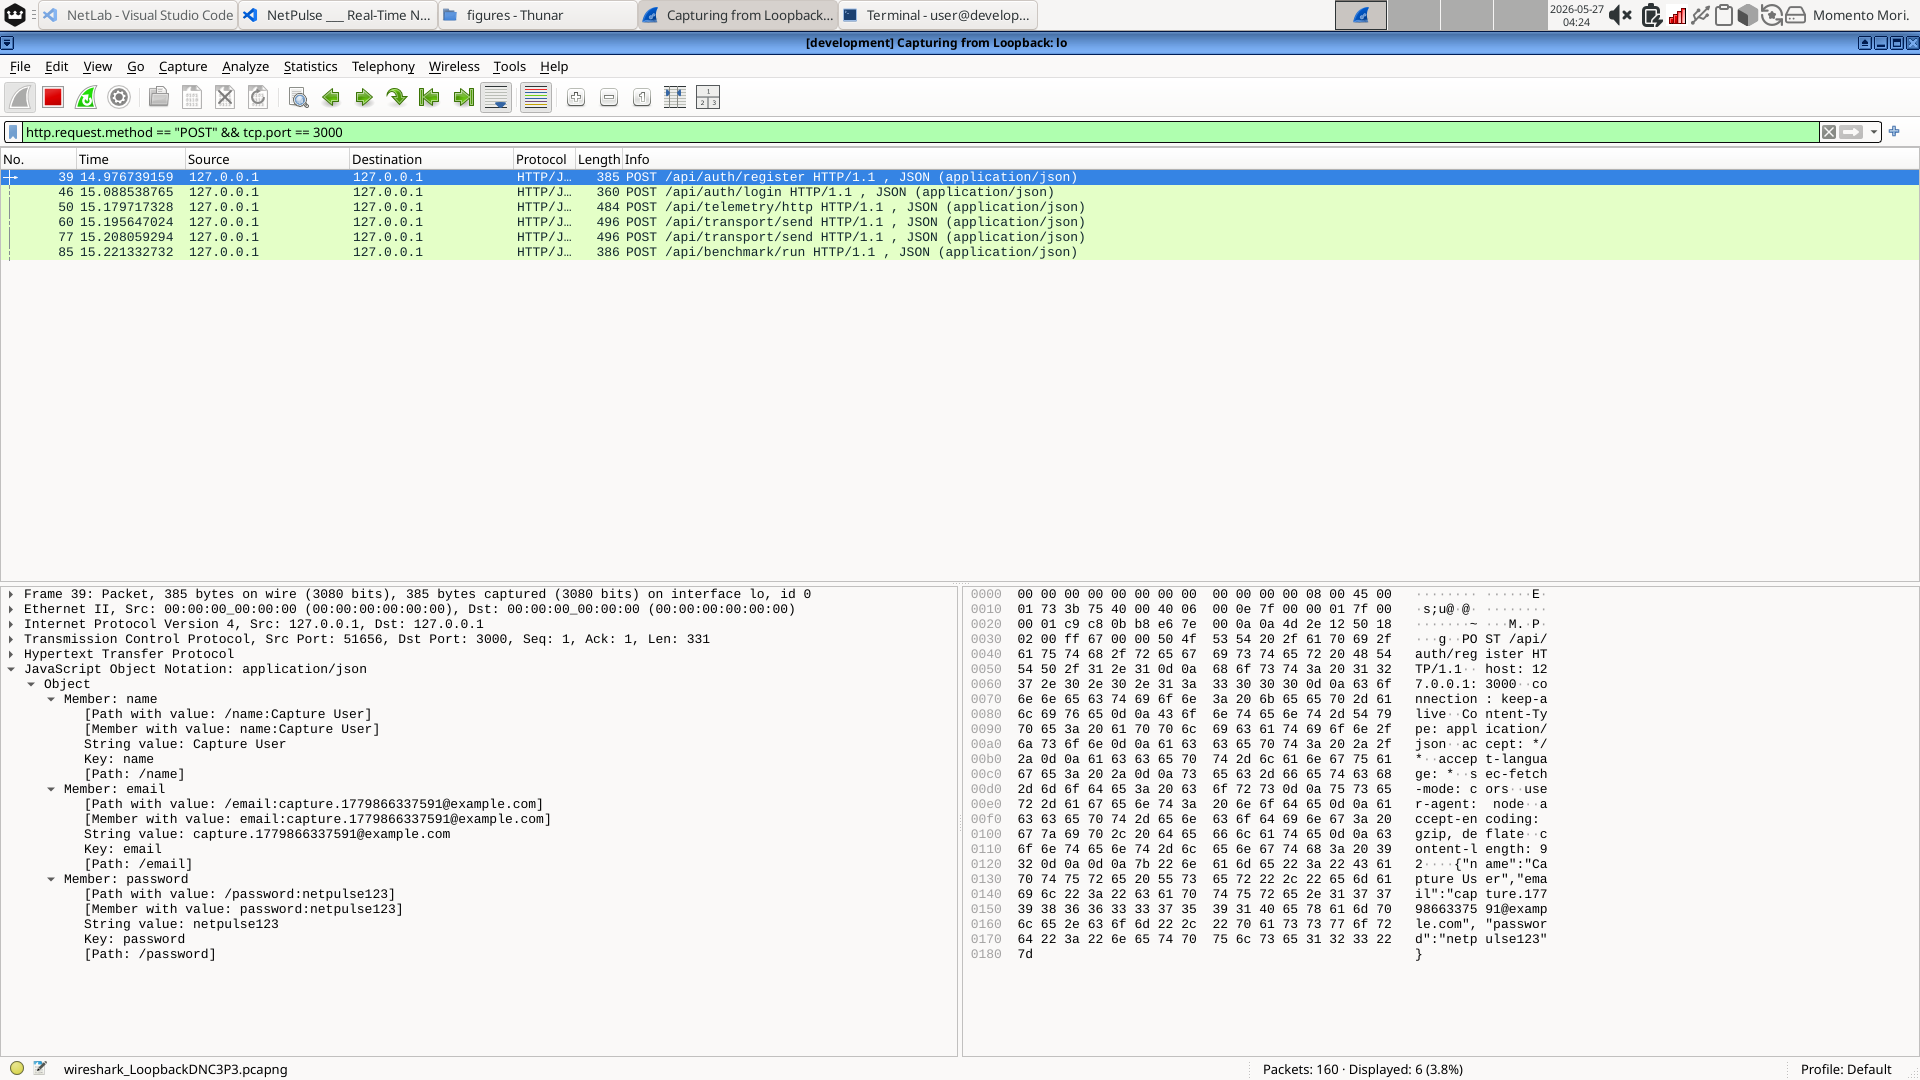
\includegraphics[width=0.98\linewidth]{figures/screenshot1.png}
\caption{Visão geral das requisições HTTP POST capturadas no loopback: registro, login, telemetria e invocações de transporte/benchmark.}\label{fig:http-posts}
\end{figure}

\begin{figure}[!htbp]
\centering
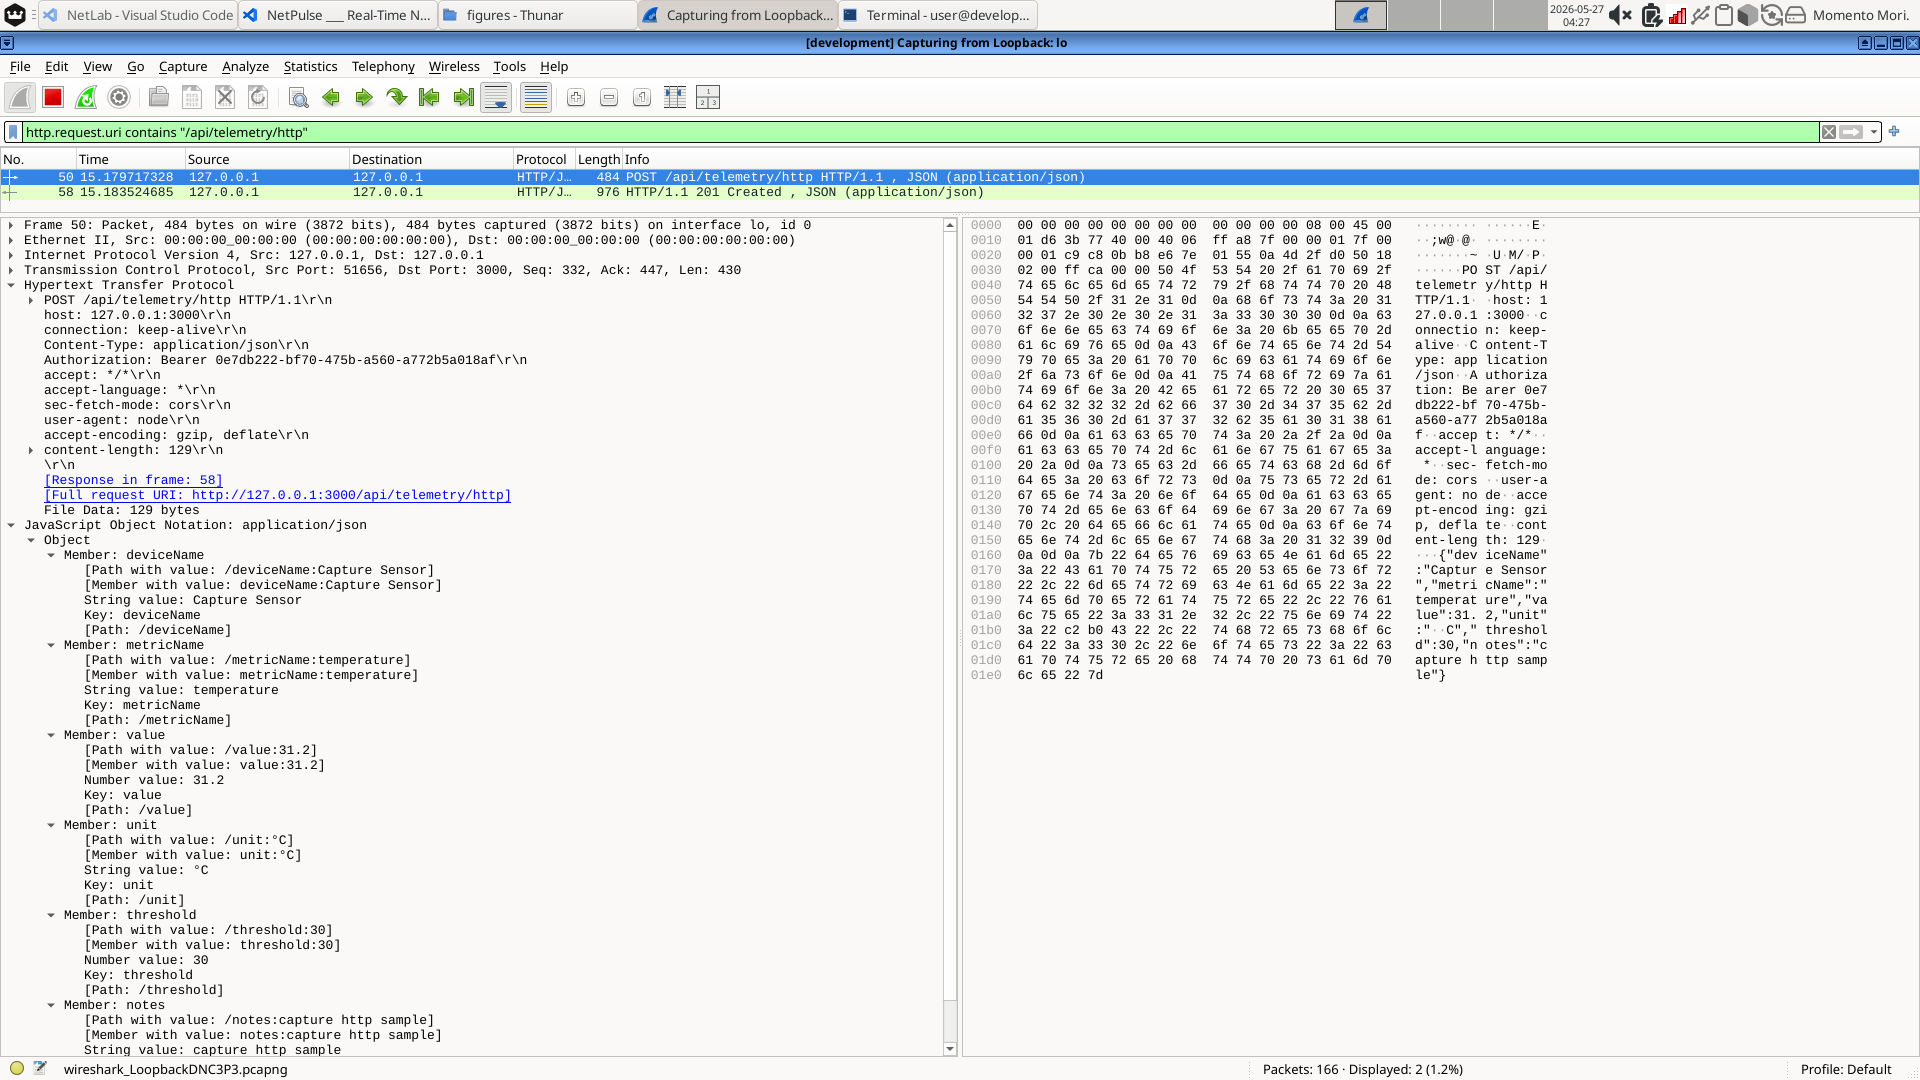
\includegraphics[width=0.98\linewidth]{figures/screenshot2.png}
\caption{Detalhe de uma requisição de telemetria HTTP para \texttt{/api/telemetry/http}: cabeçalhos, token de autorização e payload JSON do sensor.}\label{fig:telemetry-detail}
\end{figure}

\subsubsection{WebSocket em tempo real}
Após o login, o cliente abre uma conexão WebSocket para receber atualizações assíncronas. Em termos práticos, isso reduz a necessidade de polling e deixa o painel mais reativo. Na captura, o interessante é observar que a conexão permanece aberta e que o tráfego subsequente contém mensagens de controle e dados em tempo real sem o custo de abrir novos sockets para cada atualização.

\subsubsection{Handshake TCP e relays de transporte}
Na comunicação TCP, o Wireshark permite identificar o handshake de três vias, a troca de ACKs e a sequência de mensagens newline-delimited JSON.\@ O canal TCP do NetPulse foi desenhado justamente para ser simples de ler e fácil de demonstrar em aula. A figura que deve ser capturada no laboratório pode mostrar o SYN, SYN/ACK e ACK iniciais, seguidos da mensagem de telemetria e da resposta do servidor~\cite{wireshark}.

\begin{figure}[!htbp]
\centering
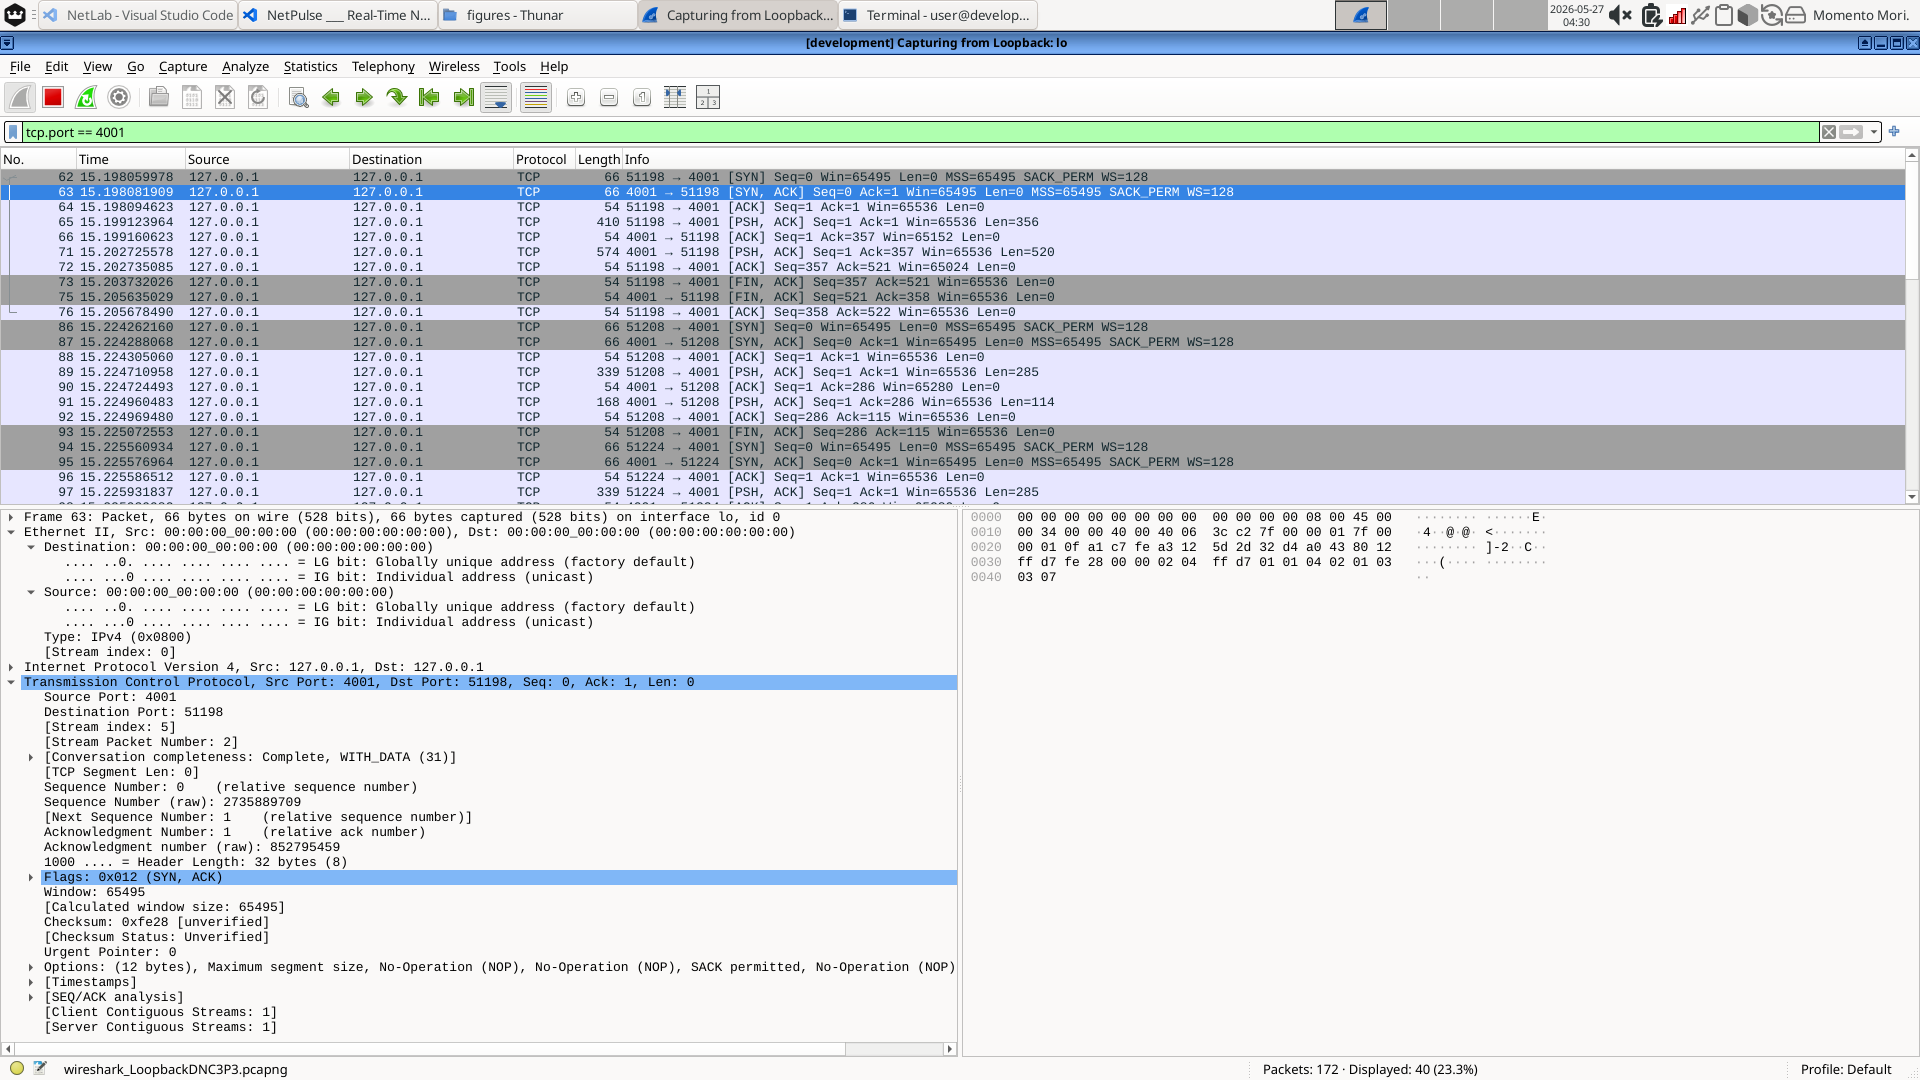
\includegraphics[width=0.98\linewidth]{figures/screenshot3.png}
\caption{Captura Wireshark do relay TCP (porta~4001): mostra o handshake TCP (SYN, SYN/ACK, ACK) seguido do pacote de telemetria e da confirmação do servidor.}\label{fig:tcp-capture}
\end{figure}

\subsubsection{Pacotes UDP}
O canal UDP foi utilizado para mostrar um comportamento mais enxuto e sem estabelecimento de conexão. Em uma análise local, a troca consiste em datagramas únicos de ida e volta. Esse canal é útil para discutir perdas, ausência de retransmissão e menor overhead. Mesmo em loopback, a diferença estrutural entre TCP e UDP permanece visível na captura~\cite{wireshark}.

\begin{figure}[!htbp]
\centering
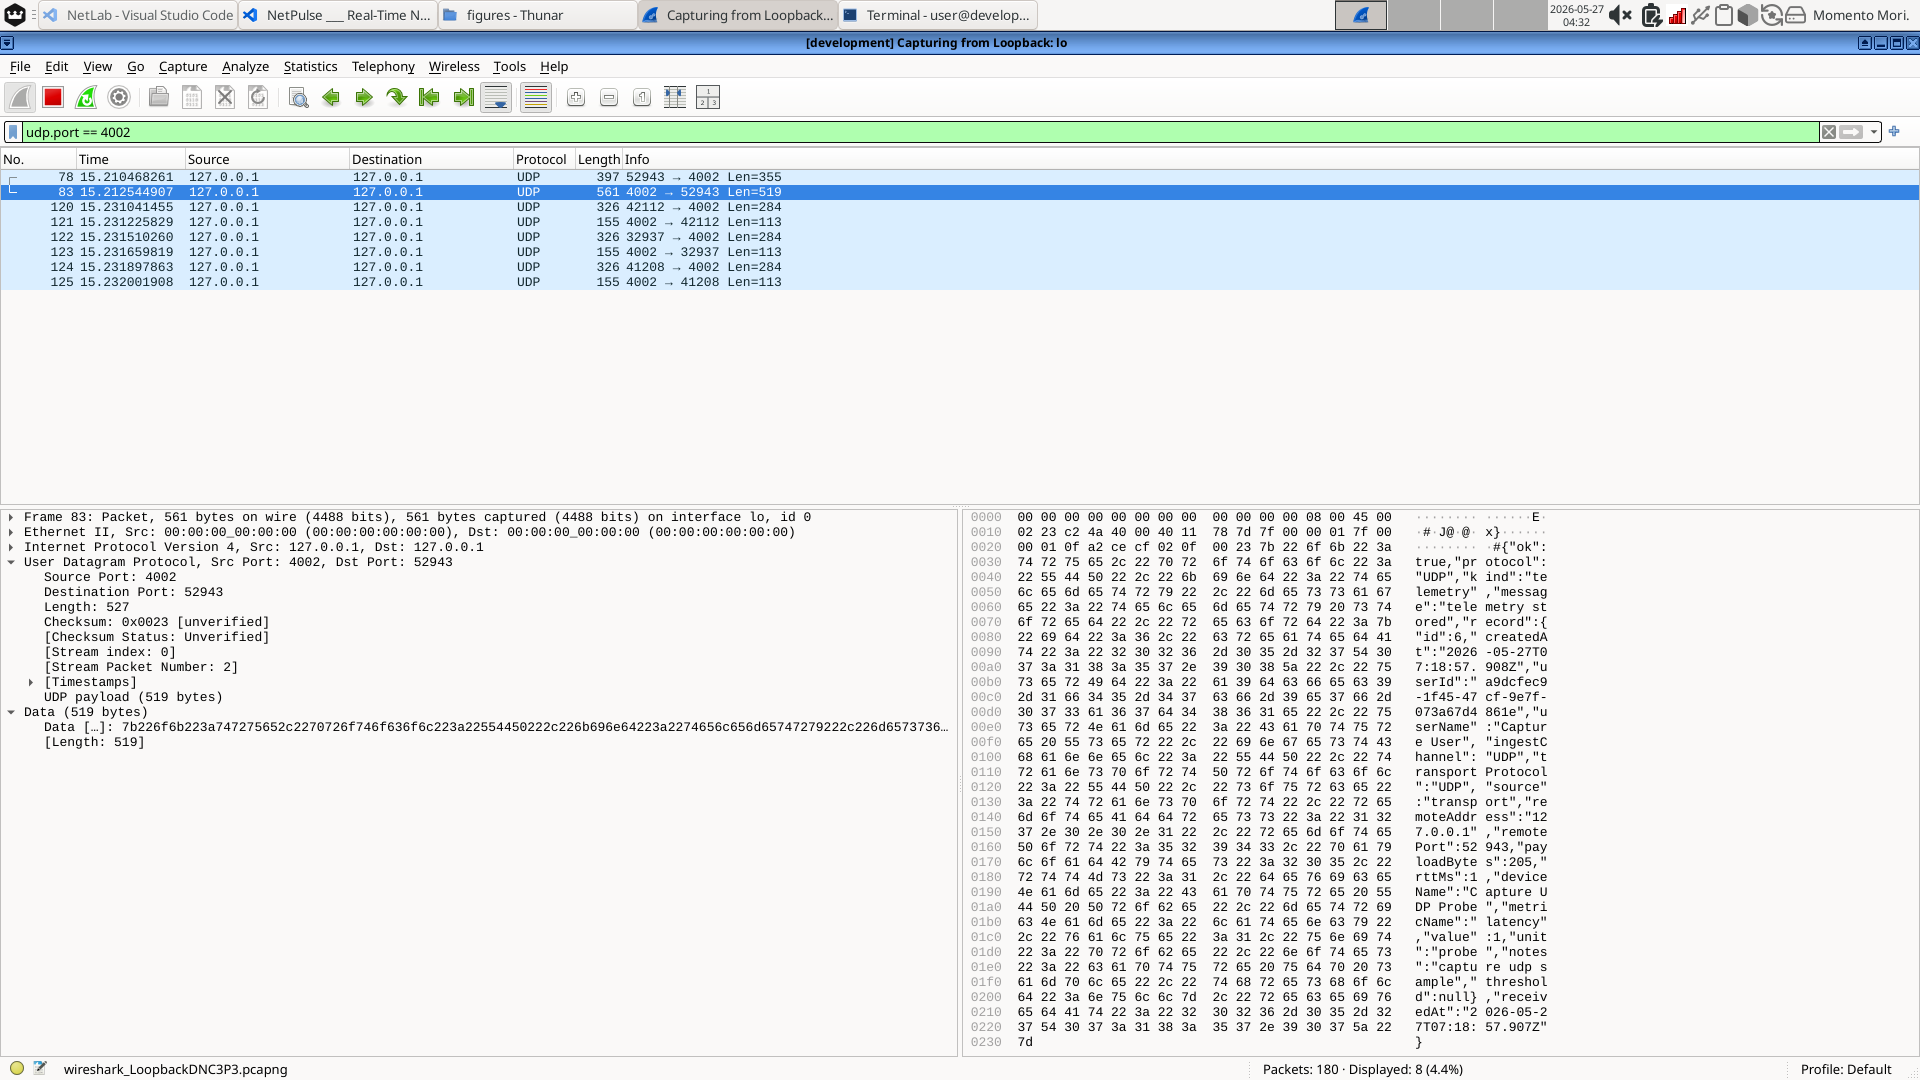
\includegraphics[width=0.98\linewidth]{figures/screenshot4.png}
\caption{Captura Wireshark do relay UDP (porta~4002): datagrama único contendo JSON em texto claro e a resposta de confirmação do servidor.}\label{fig:udp-capture}
\end{figure}

\subsubsection{RTT, throughput e comparação}
\begin{figure}[!htbp]
\centering
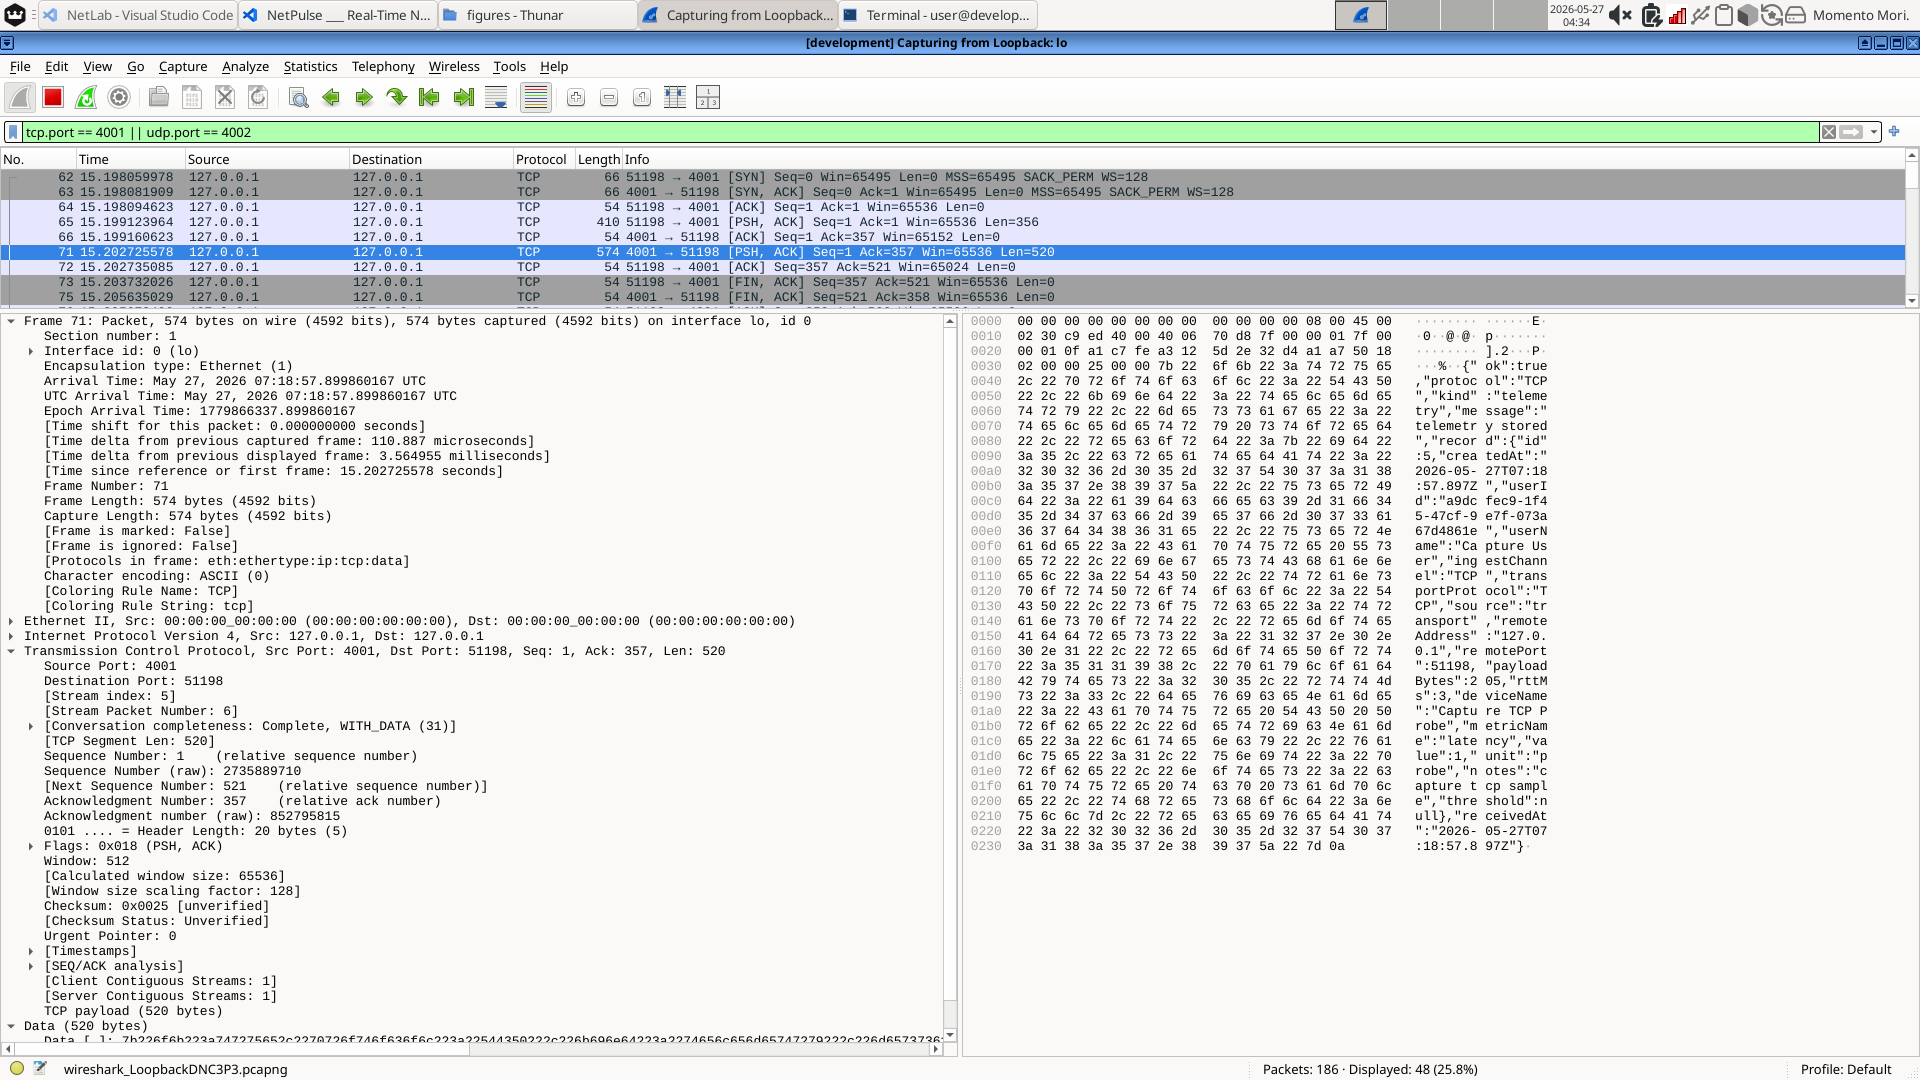
\includegraphics[width=0.98\linewidth]{figures/screenshot5.png}
\caption{Comparativo lado-a-lado de fluxos TCP e UDP capturados: sequência de handshakes e PSH de um fluxo TCP (porta~4001) e datagramas UDP do transporte (porta~4002) mostrando payloads de telemetria.}\label{fig:tcp-udp-compare}
\end{figure}

\begin{table}[!htbp]
\centering
\caption{Campos a registrar na análise experimental}\label{tab:metrics}
\begin{tabular}{p{2.5cm} p{3.9cm}}
\toprule
\textbf{Métrica} & \textbf{Observação esperada}\\
\midrule
RTT & Tempo de ida e volta entre cliente e servidor\\
Throughput & Vazão estimada em Mbps\\
Tamanho do pacote & Bytes por mensagem transmitida\\
Retransmissão & Esperada principalmente em TCP sob perda\\
Perda UDP & Pode ocorrer em cenários reais de congestão\\
\bottomrule
\end{tabular}
\end{table}

\subsubsection{Sequência cliente-servidor}
A sequência típica do sistema é: registro, login, abertura do WebSocket, envio da telemetria, geração de alerta quando aplicável e execução do benchmark. Essa cadeia permite correlacionar os conteúdos dos capítulos introdutórios de redes com a observação prática dos protocolos na pilha de comunicação.

\subsubsection{Persistência e tratamento de erros}
O NetPulse persiste usuários, tokens, telemetria, alertas, logs e resultados de benchmark em um arquivo JSON local, mantendo o mesmo formato padronizado descrito pela RFC~8259~\cite{rfc8259}. Essa decisão simplifica a reprodução do experimento, reduz a dependência de serviços externos e mantém o foco nos conceitos de comunicação em rede. Para evitar crescimento descontrolado do arquivo, o servidor mantém janelas de retenção para logs, alertas e medições mais recentes.

\section{Conclusões}
O NetPulse atendeu ao objetivo de integrar, em uma única aplicação simples, os elementos centrais solicitados no projeto: cliente web, servidor funcional, comunicação HTTP, módulo em tempo real, persistência e comparação entre TCP e UDP.\@ A arquitetura reduzida favorece estabilidade e facilita a demonstração prática.

A análise com Wireshark é especialmente rica porque a solução produz tráfego em diferentes camadas e com perfis distintos de comunicação. O HTTP atende ao fluxo principal de uso, o WebSocket mantém o painel atualizado e os relays TCP e UDP viabilizam a comparação de RTT, throughput, sequência de mensagens e tamanho dos pacotes.

Do ponto de vista pedagógico, o sistema traduz bem os conceitos de encapsulamento, segmentação, multiplexação e comunicação fim a fim. Como trabalho acadêmico, ele fornece material suficiente para relatório, apresentação e defesa oral sem exigir uma infraestrutura complexa.

Além das contribuições já mencionadas, o NetPulse provê uma base prática para experiências laboratoriais: os scripts de geração de tráfego e os testes de fumaça permitem reproduzir cenários de captura em loopback e coletar métricas comparáveis entre execuções. Isso facilita a verificação experimental em diferentes máquinas e configurações, tornando o projeto útil tanto para demonstrações em sala quanto para avaliações reproducíveis.

Reconhecem-se limitações claras — em particular, a execução em ambiente de loopback não reproduz perdas e variações reais de rede — o que recomenda complementar os experimentos com testes em redes reais ou em topologias que injetem atraso e perda controlada. Como trabalho futuro, sugere-se: (i) desacoplar os relays em processos independentes para facilitar estudo de escalabilidade; (ii) adicionar suporte opcional a um armazenamento mais robusto (por exemplo, SQLite) para avaliar comportamento em cargas maiores; e (iii) incluir scripts de reprodução automatizada para facilitar comparações entre diferentes versões do sistema.

\begin{thebibliography}{10}
\bibitem{tanenbaum} A. S. Tanenbaum and D. J. Wetherall, \emph{Computer Networks}, 5th ed. Pearson, 2011.
\bibitem{kurose} J. F. Kurose and K. W. Ross, \emph{Computer Networking: A Top-Down Approach}, 8th ed. Pearson, 2021.
\bibitem{rfc793} J. Postel, \emph{Transmission Control Protocol}, RFC 793, Sep. 1981.
\bibitem{rfc768} J. Postel, \emph{User Datagram Protocol}, RFC 768, Aug. 1980.
\bibitem{rfc9110} R. Fielding et al., \emph{HTTP Semantics}, RFC 9110, Jun. 2022.
\bibitem{rfc6455} I. Fette and A. Melnikov, \emph{The WebSocket Protocol}, RFC 6455, Dec. 2011.
\bibitem{rfc8259} T. Bray, \emph{The JavaScript Object Notation (JSON) Data Interchange Format}, RFC 8259, Dec. 2017.
\bibitem{rfc2544} S. Bradner and J. McQuaid, \emph{Benchmarking Methodology for Network Interconnect Devices}, RFC 2544, Mar. 1999.
\bibitem{wireshark} Wireshark Foundation, \emph{Wireshark User's Guide}, available at \url{https://www.wireshark.org/docs/}.
\end{thebibliography}

\end{document}
